%%%%%%%%%%%%%%%%%%%%%%%%%%%%%%%%%%%%%%%%%%%%%%%%%%%%%%%%%%%%%%%%%%%%%%%%%%
%%%%%                         CHAPITRE 1                            %%%%%%
%%%%%%%%%%%%%%%%%%%%%%%%%%%%%%%%%%%%%%%%%%%%%%%%%%%%%%%%%%%%%%%%%%%%%%%%%%

\lhead[\fancyplain{}{\leftmark}]%Pour les pages paires \bfseries
      {\fancyplain{}{}} %Pour les pages impaires
\chead[\fancyplain{}{}]%
      {\fancyplain{}{}}
\rhead[\fancyplain{}{}]%Pour les pages paires 
      {\fancyplain{}{\rightmark}}%Pour les pages impaires \bfseries
\lfoot[\fancyplain{}{}]%
      {\fancyplain{}{}}
\cfoot[\fancyplain{}{\thepage}]%\bfseries
      {\fancyplain{}{\thepage}} %\bfseries
\rfoot[\fancyplain{}{}]%
     {\fancyplain{}{\scriptsize}}


%%%%%%%%%%%%%%%%%%%%%%%%%%%%%%%%%%%%%%%%%%%%%%%%%%%%%%%%%%%%%%%%%%%%%%%%%%
%%%%%                      Start part here                          %%%%%%
%%%%%%%%%%%%%%%%%%%%%%%%%%%%%%%%%%%%%%%%%%%%%%%%%%%%%%%%%%%%%%%%%%%%%%%%%%

\chapter{State of the art}
\label{ch:1}

%======================================================	Résumé du chapitre

\begin{center}
\rule{0.7\linewidth}{.5pt}
\begin{minipage}{0.7\linewidth}
\smallskip

\textit{Motion capture (MoCap) in sports is traditionally performed with marker-based (opto-electronic) systems. However, this presents some drawbacks. As a consequence, alternatives are being investigated, among which those offered by Inertial Measurement Units (IMUs) or dept-field (RGB-D) cameras. Markerless analysis from videos sources represents one of the most promising prospects, which has been possible thanks to progress in machine learning. From 2D pose estimation to 3D joint angle determination, this is a new field which opens up new possibilities for motion analysis in a sports context.\newline \newline
This chapter is an up-to-date and more detailed version of the introduction of the previously published paper: "Pose2Sim: An End-to-End Workflow for 3D Markerless Sports Kinematics—Part 1: Robustness" \cite{Pagnon2021}. }

%\smallskip
\end{minipage}
\smallskip
\rule{0.7\linewidth}{.5pt}
\end{center}

\minitoc
\newpage



\FloatBarrier
\section{Overall context of kinematics in sports}
\subsection{General context}

As coaching athletes implies observing and understanding their movements, motion capture (MoCap) is essential in sports. It helps improving movement efficiency, preventing injuries, or predicting performances. For the last few decades, marker-based systems have been considered the best choice for the analysis of human movement, when regarding the trade-off between ease of use and accuracy. However, these methods have proven to be much more challenging in a sports context than in a laboratory setting, and to be generally inappropriate \cite{Mündermann2006, Colyer2018}. As a consequence, other methods have been investigated (see Table~\ref{table:tab_stateart}).

\subsection{Marker-based systems}

Marker-based systems use a network of opto-electronic cameras. Each of these cameras are surrounded by a crown of infrared LEDs, which projects light toward the subject, who is equipped with reflective markers. Ideally, only the light reflected from these markers is captured by the cameras. The camera usually pre-processes the image to make it binary, and only outputs the coordinates of the detected marker (Figure~\ref{fig_mk1}). 

\begin{figure}[hbtp]
	\centering
	\begin{subfigure}[b]{1\textwidth}
		\centering
		\def\svgwidth{\columnwidth}
		\fontsize{10pt}{10pt}\selectfont
		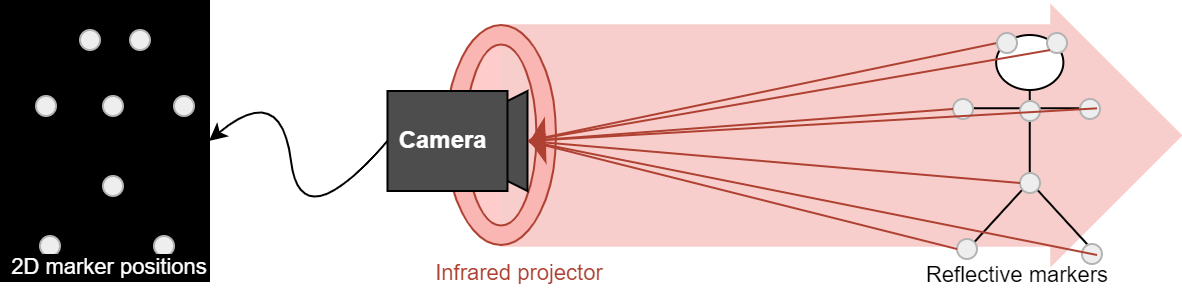
\includegraphics[width=\linewidth]{"../Chap1/Figures/Markers_1.png"}
		\caption{An opto-electronic camera is traditionnally surrounded by a crown of infrared LEDs, projecting light toward the subject. The subject wears markers, which reflect light back to the camera. Marker positions are then known in the camera plane.}
		\label{fig_mk1}
	\end{subfigure}
	\qquad
	\begin{subfigure}[b]{1\textwidth}
		\centering
		\def\svgwidth{\columnwidth}
		\fontsize{10pt}{10pt}\selectfont
		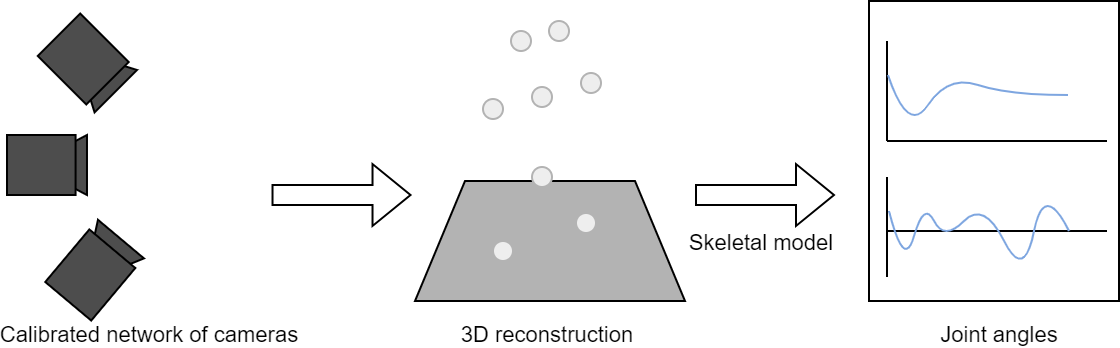
\includegraphics[width=\linewidth]{"../Chap1/Figures/Markers_2.png"}
		\caption{Once calibrated, a network of these cameras allows for 3D reconstruction of marker positions. Marker coordinates are then used to infer the posture of the subject.}
		\label{fig_mk2}
	\end{subfigure}
	\caption{Principles of marker-based motion capture. (Figure~\ref{fig_mk1}) presents the functioning of an opto-electronic camera. (Figure~\ref{fig_mk2}) shows how a network of calibrated motion capture cameras helps obtaining joint angles.}
	\label{fig_mk}
\end{figure}

If calibrated, using a network of these cameras allows for triangulating the 2D coordinates. Calibration involves knowing the cameras' intrinsic properties (such as focal length, optical center, distortion) as well as their extrinsic properties (their position and orientation as regards to the global coordinate system.) See Chapter 2.2 on \nameref{sec:3D reconstruction} for more details. The reconstructed 3D marker positions are then used to optimize the posture of a physically consistent skeleton, scaled to each individual subject. In particular, this allows for obtaining 3D joint angles at each point in time, commonly referred to as inverse kinematics (IK.)
% allows for 2 fois

Yet, reflective marker-based camera systems are complex to set up, are time-consuming, and are very expensive. They also require specific lightning conditions, and involve cumbersome cabling. Moreover, markers may fall off the body of the participant due to sharp accelerations or sweat. They can hinder the natural movement of athletes, which is likely to affect their warm-up, focus, and safety. While the accuracy of landmark location is claimed to be sub-millimetric in marker-based methods \cite{Topley2020}, marker placement is tedious, intrusive, prone to positioning variability from the operator \cite{Tsushima2003}, and subject to skin movement artifacts, especially on soft tissues. Della Croce et al. found out that inter-operator variations in marker placements range from 13 to 25 mm, which can propagate up to 10\degree{} in joint angle prediction \cite{Gorton2009,Croce1999}. For example, tissue artifacts account for up to a 2.5 cm marker displacement at the thigh, which can cause as much as a 3\degree{} error in knee joint angles tissues \cite{Benoit2015,Cappozzo1995}. Joint positions must be calculated explicitly in marker-based methods, which introduces more variability: these errors range up to 5 cm, which can contribute up to 3\degree{} of error in lower limb joint angles \cite{Leboeuf2019}. Nevertheless, since marker-based methods benefit from decades of research, they are still considered as the reference method for motion capture.

\FloatBarrier
\subsection{IMU and RGB-D systems}

Consequently, other approaches based on alternative technologies have been investigated over the past years. For instance, wearable Inertial Measurement Units (IMUs) can be placed on an athlete's limbs. IMUs are generally made of an accelerometer, a gyroscope, and a magnetometer. The accelerometer measures the linear acceleration, the gyroscope measures the rotational speed, and the magnetometer measures the orientation of the earth magnetic field. Fusing and integrating these signals allows for the determination of their 3D orientations. The orientation of the athlete's limbs can then be used in combination with a skeletal model to infer their posture (Figure~\ref{fig_imus}).

IMUs offer the advantages of getting away from all camera-related issues. They are inexpensive, they do not involve any complex setup and calibration, the field of view is larger, data do not take much storage space, they are not sensitive to self- and gear-occlusions, they can be operated outside of a controlled environment, and they can work in real-time \cite{Johnston2019,Chambers2015}. They still have the drawback of requiring an external equipment to wear, involving high technical skills from the operator, and are sensitive to ferromagnetic disturbances. Above all, they are exposed to drift over time and need to be calibrated every few minutes. Joint angle accuracy is relatively good in the flexion/extension plane, but less so in other rotational planes where errors are greater than 5\degree{} for most motions \cite{Zhang2013, Rekant2022}. Moreover, they are not suitable for joint positions assessment, since these are obtained through multiple integrations of the original signal \cite{Ahmad2013}. 

\begin{figure}[hbtp]
	\centering
	\def\svgwidth{1\columnwidth}
	\fontsize{10pt}{10pt}\selectfont
	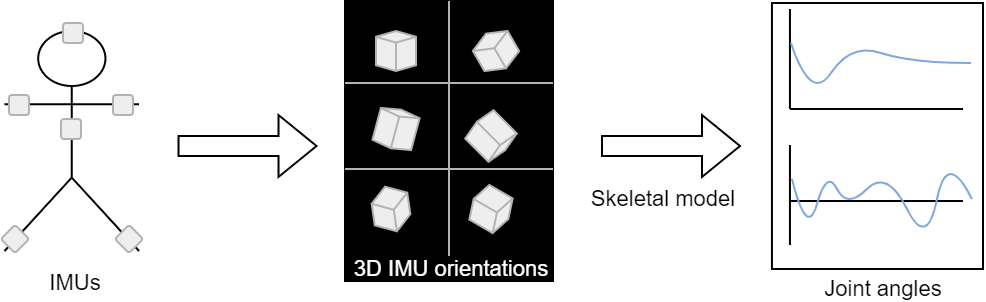
\includegraphics[width=\linewidth]{"../Chap1/Figures/IMUs.png"}
	\caption{IMUs are placed on the subject's limbs. The orientation of the limbs is then used to infer the posture of the subject.}
	\label{fig_imus}
\end{figure}
\FloatBarrier

Another approach involves depth-field cameras (RGB-D). Older models projected infrared \textit{structured} light (i.e., a pattern) onto the scene. The relative deformation of the pattern reflected from the scene was then used to estimate depth. Newer models project infrared \textit{modulated} light onto the scene. The time of flight of the light reflected from the scene is then used to estimate depth. Results are commonly considered to be 2.5D, since only the depth of the front facing plane of view is measured. Gait analysis results are natively poor, but after an optimization by a neural network, \cite{Guo2022} manage to get root-mean-square errors under 7° for knee flexion/extension angle at the most challenging part of the gait cycle, although 3D joint angle errors usually stay under 2-3°. However, it may not perform as well on other motions on which the neural network has not been trained. A network of a few RGB-D cameras can give access to full 3D \cite{Carraro2017,Choppin2013,Colombel2020}. Nevertheless, these cameras hardly function in direct sunlight nor at a distance over 5 meters, and they work at lower frame rates (generally under 30 Hz) \cite{Han2013, Pagliari2015}. 

\begin{figure}[hbtp]
	\centering
	\def\svgwidth{1\columnwidth}
	\fontsize{10pt}{10pt}\selectfont
	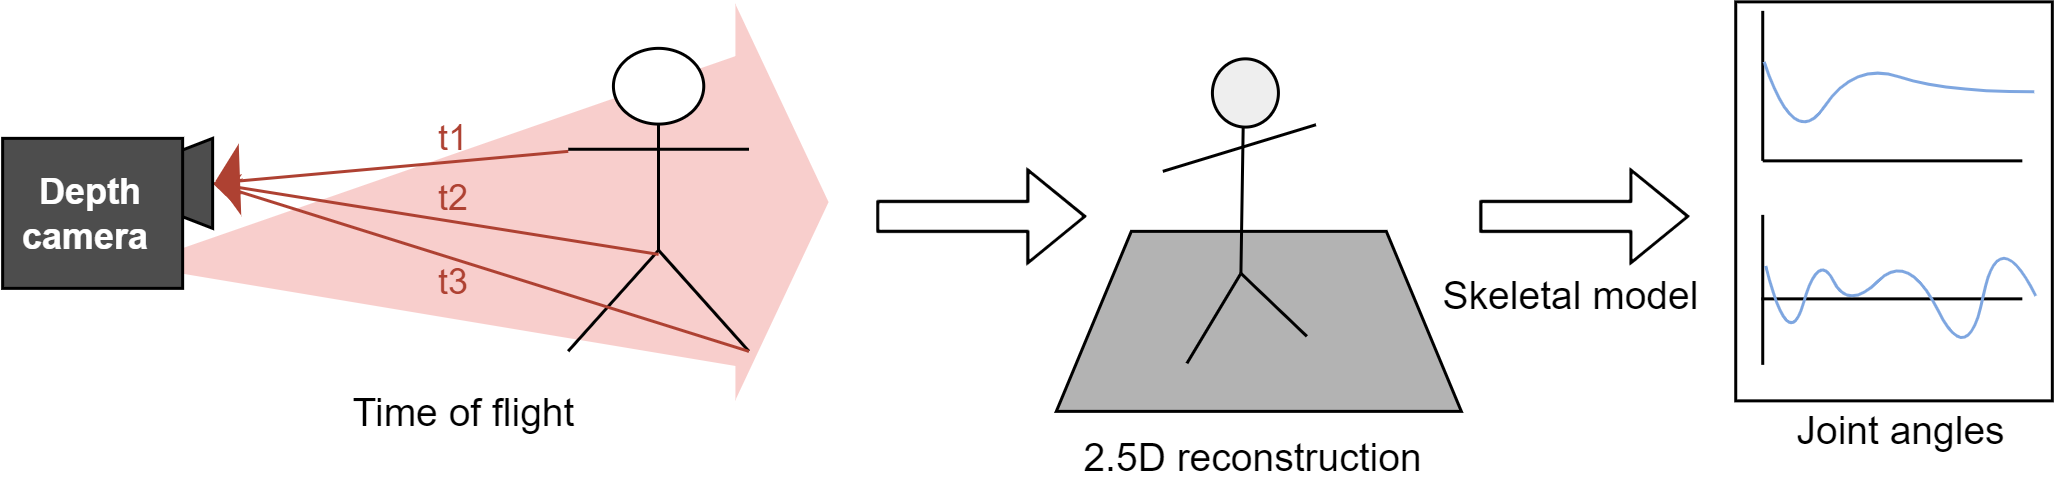
\includegraphics[width=\linewidth]{"../Chap1/Figures/Depth.png"}
	\caption{A depth-field camera (RGB-D) projects infrared modulated light onto the subject's body. The time it takes for the light to be reflected to the camera sensor (time of flight) depends on distance, and gives access to the depth of the scene.	Older RGB-D cameras use structured light rather than time of flight calculations to infer depth.}
	\label{fig_depth}
\end{figure}

\FloatBarrier
\subsection{Markerless systems}

A recent breakthrough has come from computer vision, and the advent of 2D pose estimation from image sources, which quickly became more efficient and accurate. The explosion of deep-learning based methods from camera videos, for which the research has skyrocketed around 2016 \cite{Wang2021a}, is related to the increase in storage capacities and huge improvements in GPU computing. A search on the ScienceDirect database for “deep learning 3D human pose estimation” produced fewer than 100 papers per year until 2015, and the number is now reaching over 1,000, fitting an exponential curve (Figure~\ref{fig_exp}).


\begin{figure}[hbtp]
	\centering
	\def\svgwidth{1\columnwidth}
	\fontsize{10pt}{10pt}\selectfont
	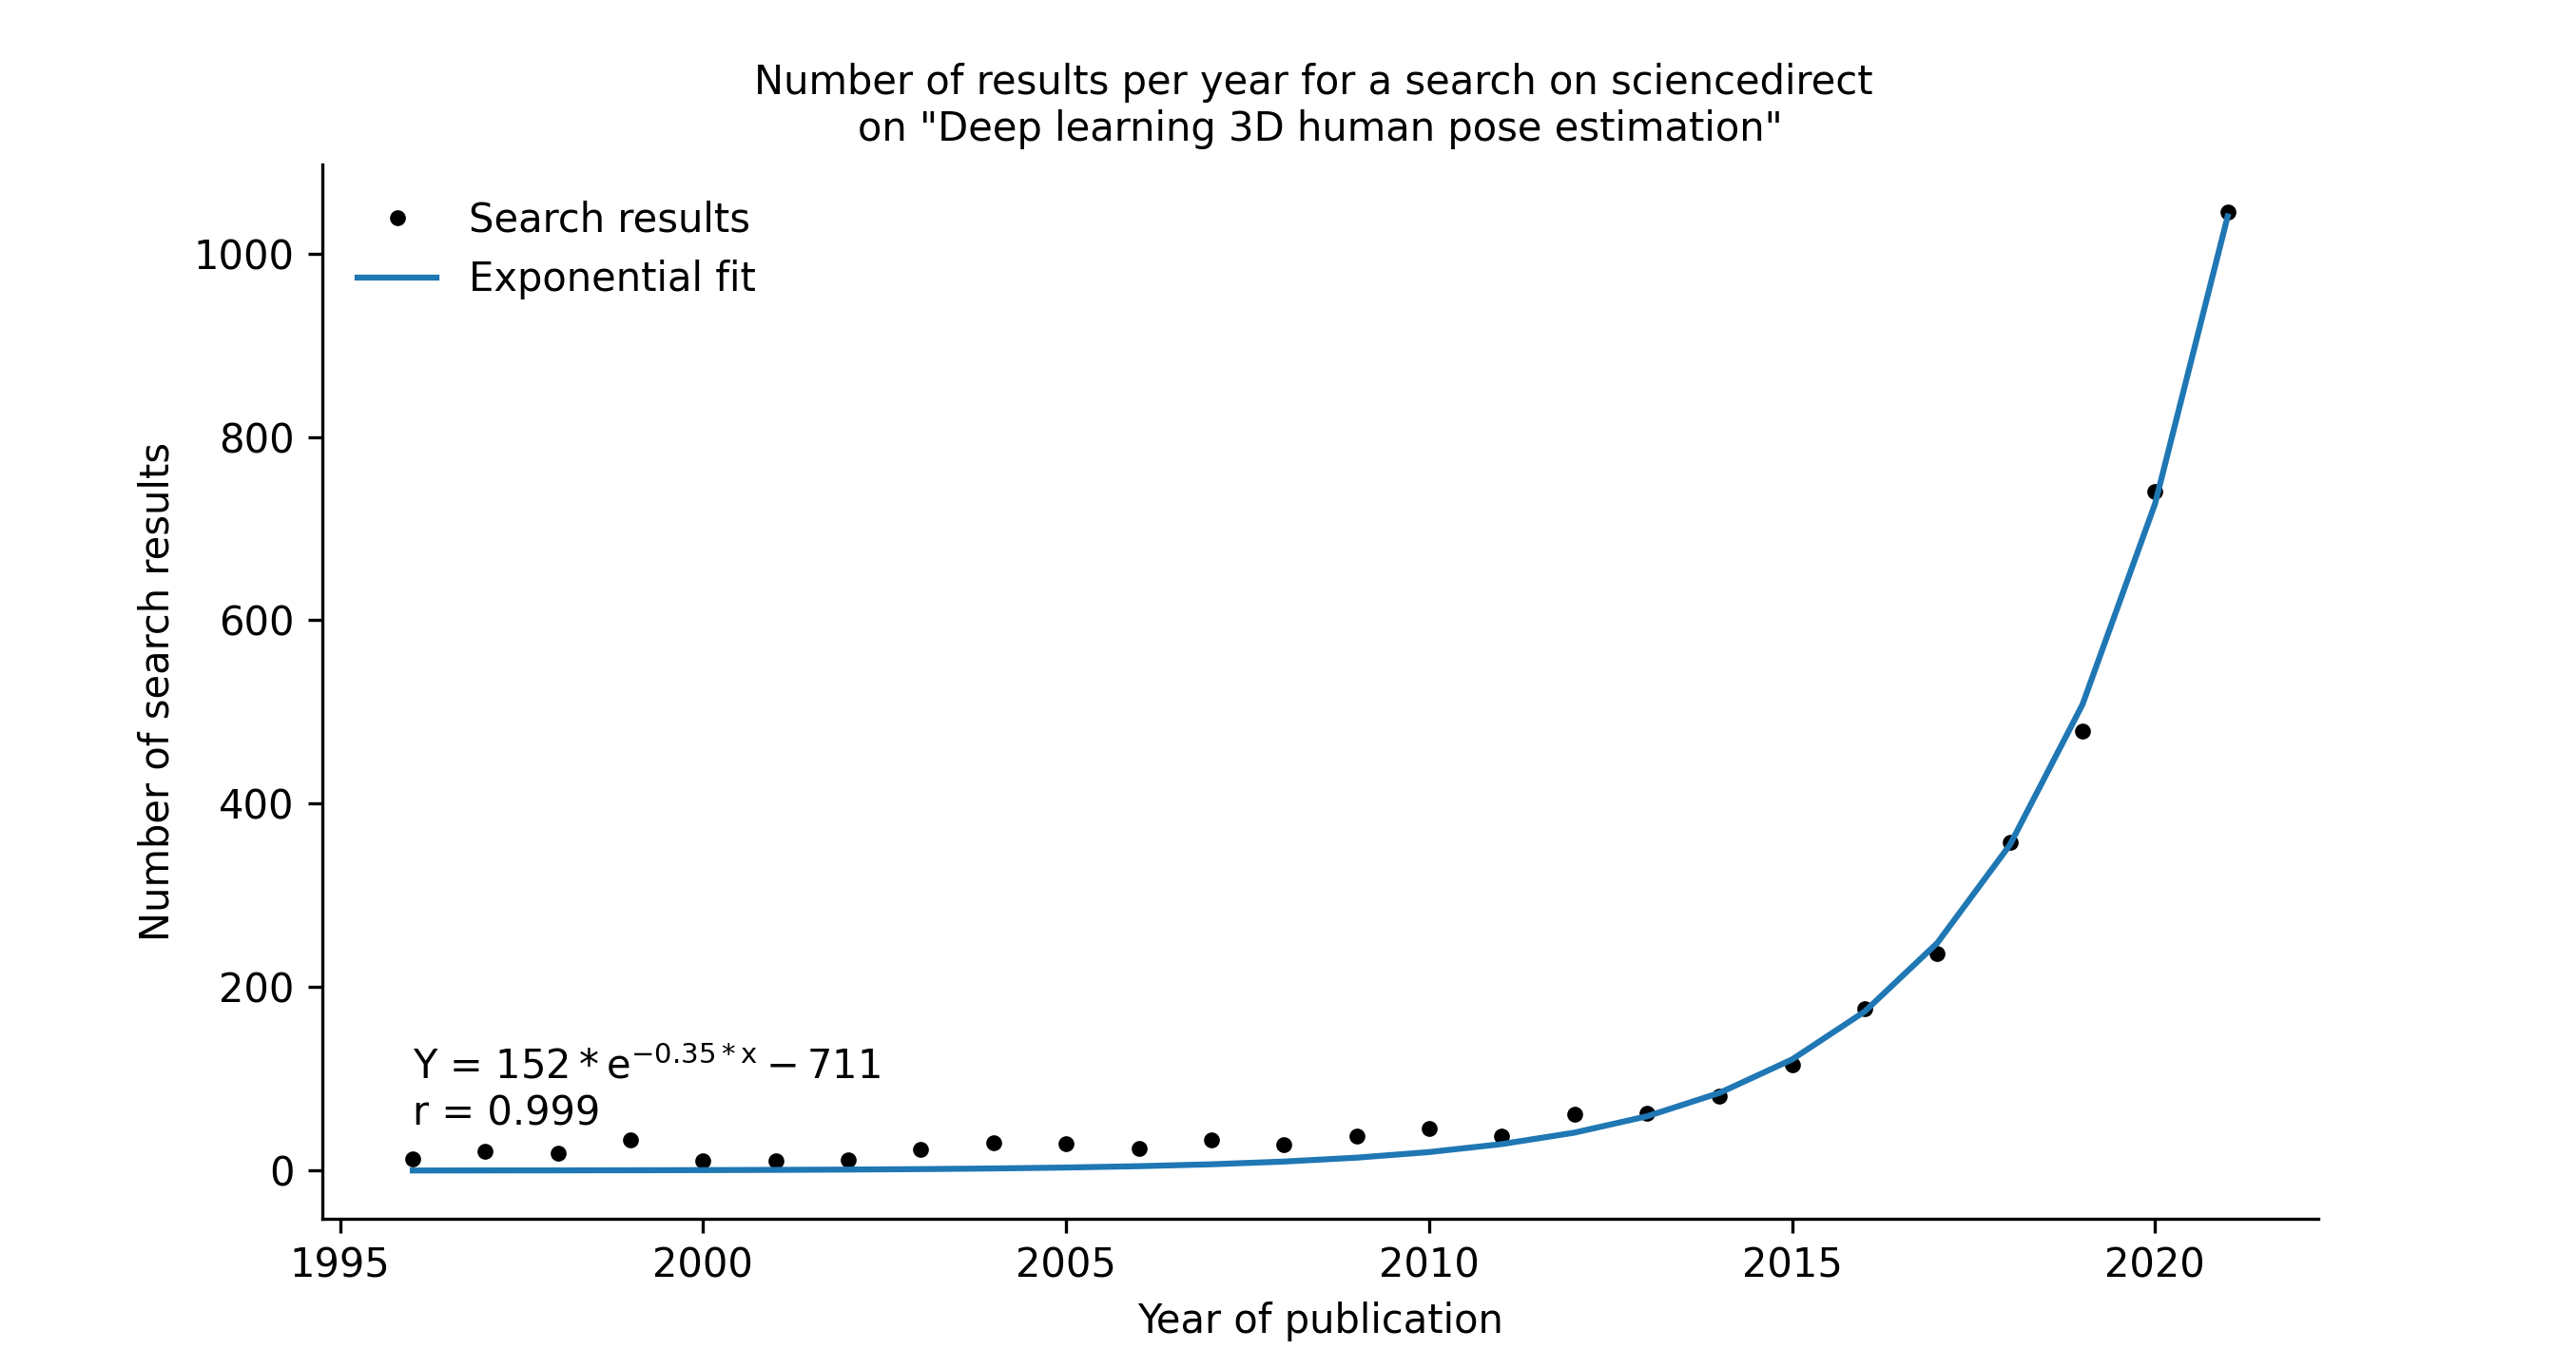
\includegraphics[width=\linewidth]{"../Chap1/Figures/Fig_exp.png"}
	\caption{The search for “deep learning 3D human pose estimation” (dots) fits an exponential curve (line). The search produced less than 100 results until 2015, and is now well over a 1,000 per year.}
	\label{fig_exp}
\end{figure}

It has rekindled interest from the biomechanics community towards image-based motion analysis, which is where it all started with the invention of chronophotography in the 19th century by Marey in France, and Muybridge in the USA \cite{Baker2007}. Currently, two approaches coexist in human and animal motion analysis: the first one mostly focuses on joint positions, and is lead by the computer vision and the deep-learning communities; while the second one is interested in joint angles, such as the biomechanics community uses to obtain physically coherent kinematics individualized to each subject. One of the main current challenges is to bridge the gap between these two worlds, and to take advantage of deep-learning technologies for kinematic analysis \cite{Cronin2021,Seethapathi2019}. 

\FloatBarrier
\section{2D markerless analysis}
\subsection{2D pose estimation}

The most well-known off-the-shelf 2D human pose estimation solutions are OpenPose \cite{Cao2019} (Figure~\ref{fig_openpose}), and to a lesser extent AlphaPose \cite{Fang2017}. While both show similar accuracy, AlphaPose is faster when few people are in the scene. However, OpenPose has the advantage of being a bottom-up approach, whose computational cost does not increase with the number of persons detected \cite{Cao2019}. It is also more widespread (25,000 stars on the GitHub repository, vs. 6,000 for AlphaPose). A bottom-up approach first detects all available joint keypoints, and then associates them to the right persons; while a top-bottom approach first detects bounding boxes around each person, and then finds joint keypoints inside of them. OpenPose is the only multi-person 2D pose estimation solution that provides foot keypoints, which are essential for sports motion analysis.

Other approaches have shown even better results on evaluation datasets (see review \cite{Chen2020}), but they are generally slower and not as widespread. The technology, however, is still maturing and some light-weight systems such as BlazePose \cite{Bazarevsky2020}, UULPN \cite{Wang2022a}, or YOLOv7 \cite{Wang2022b} are being proposed, which can operate in real time on a mobile phone; however, they either support single-person detection only, are not accurate enough for quantitative motion analysis \cite{Mroz2021}, or haven't been embraced by the community yet. Some work has also been done on temporal consistency across frames with OpenPifPaf, which makes the system much faster, and helps it perform better on low-resolution regime or with occlusions such as in crowds \cite{Kreiss2021}.

Two other 2D pose estimation toolboxes are DeepLabCut \cite{Mathis2018,Lauer2022} and SLEAP \cite{Pereira2022}, which were initially intended for markerless animal pose estimation. They have the advantage that they can be custom trained for the detection of any human or not human keypoint with a relatively small dataset. 

All the tools presented in this section are open-source. See Chapter 2.1.3 on \nameref{sec:Machine learning for 2D pose detection} for more technical details on their architecture.

\begin{figure}[hbtp]
	\centering
	\def\svgwidth{1\columnwidth}
	\fontsize{10pt}{10pt}\selectfont
	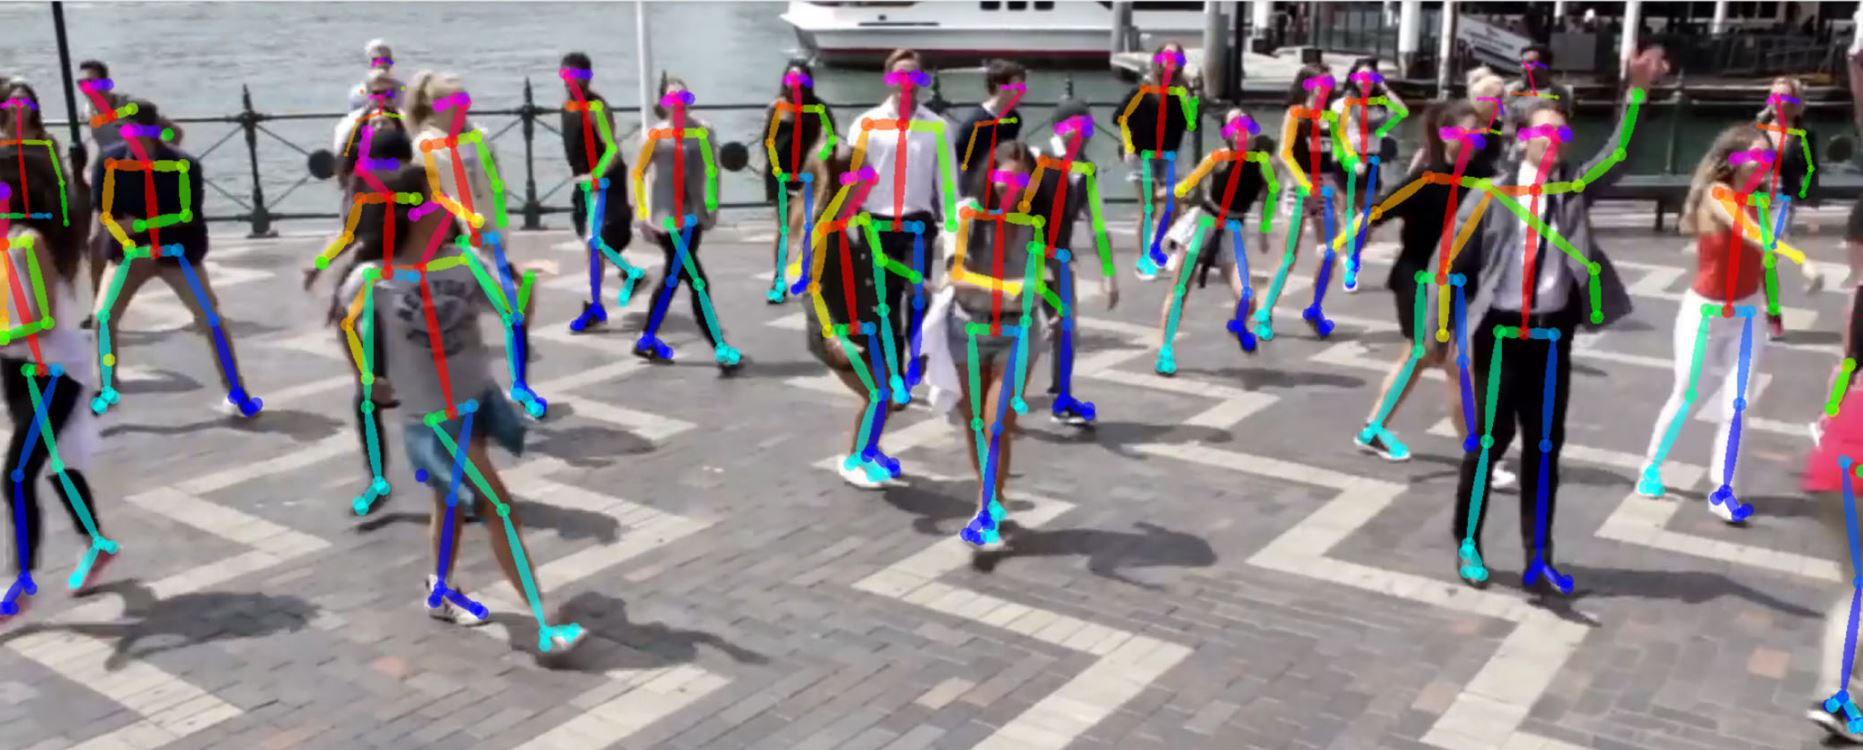
\includegraphics[width=\linewidth]{"../Chap1/Figures/OpenPose.JPG"}
	\caption{2D pose estimation by OpenPose. Image courtesy of \cite{Cao2019}.}
	\label{fig_openpose}
\end{figure}

\newpage

\subsection{2D kinematics from 2D pose estimation}

Some authors bridge 2D pose estimation to more biomechanically inspired variables, such as in gait kinematics analysis. Kidzinski et al. present a toolbox for quantifying gait pathology that runs in a Google Colab \cite{Kidziński2020}. Stenum et al. evaluate gait kinematics calculated from OpenPose input concurrently with a marker-based method. Mean absolute error of hip, knee and ankle sagittal angles were 4.0\degree{}, 5.6\degree{} and 7.4\degree{} \cite{Stenum2021}. Liao et al. have not released their code, but they use OpenPose outputs to train a model invariant to view \cite{Liao2020}. Viswakumar et al. perform direct calculation of the knee angle from an average phone camera processed by OpenPose \cite{Viswakumar2019}. They show that OpenPose is robust to challenging clothing such as large Indian pants, as well as to extreme lightning conditions. Other sports activities have been investigated, such as lower body kinematics of vertical jump \cite{Drazan2021} or underwater running \cite{Cronin2019}. Both works train their own model with DeepLabCut. Serrancoli et al. fuse OpenPose and force sensors to retrieve joint dynamics in a pedaling task \cite{Serrancolí2020}. Although it doesn't specifically use deep-learning approaches, another noteworthy tool for 2D sports movement analysis is Kinovea \cite{Fernandez2020}. It allows to manually label keypoints on a frame, and track them in time in order to obtain point trajectories or angle data. 


\FloatBarrier
\section{3D markerless analysis} 
\subsection{3D pose estimation}

There are a lot of different approaches for markerless 3D human pose estimation, and listing them all is beyond our scope (see review \cite{Wang2021a}). Some more ancient ones are not based on deep-learning and require specific lightning and background conditions, such as visual-hull reconstruction \cite{Ceseracciu2014}. Some directly lift 3D from a single 2D camera (see review \cite{Liu2022b}), with different purposes: one estimates the positions of a set of keypoints around the joint instead of determining only the joint center keypoint, so that axial rotation along the limb is solved \cite{Fisch2020}; SMPL and its sequels retrieve not only joint positions and orientations, but also body shape parameters \cite{Loper2015}; while XNect primarily focuses on real time \cite{Mehta2020}. A few approaches even strive to estimate 3D dynamics and contact forces from a 2D video input \cite{Li2019,Rempe2021,Louis2022}. Some incorporate kinematic priors into their neural networks in order to take advantage of human knowledge \cite{Xu2020a}. Surprisingly, this does not seem to be done in multi-view approaches. Rempe et al. solve occlusions from a 2D input \cite{Rempe2020}, but this remains a probabilistic guess that may be unsuccessful in case of unconventional positions of hidden limbs, whereas using more cameras would have given more trustworthy results. 

Some research attempts to solve 3D pose estimation from a network of uncalibrated cameras, i.e., cameras whose extrinsic parameters (translation and rotation with respect to the coordinate system), intrinsic parameters (focal length, pixel size, etc.), and distortion coefficients are not known (See Chapter 2.2 on \nameref{sec:3D reconstruction} for more details.) It either uses 2D pose estimations of each view as visual cues to calibrate on \cite{Takahashi2018, Xu2021, Liu2022a}, or an adversarial network that predicts views of other cameras, compares them to real views, and adjusts its calibration accordingly \cite{Ershadi-Nasab2021}. Dong et al. recover 3D human motion from unsynchronized and uncalibrated videos of a repeatable movement found on internet videos (such as a tennis serve performed by a celebrity) \cite{Dong2020}. Using uncalibrated videos is still a very experimental trend, that would require more research before being used in biomechanics.

We choose to focus on the methods that estimate 3D pose by triangulating 2D pose estimations from a network of multiple calibrated cameras. The classical evaluation metric is the MPJPE (Mean Per Joint Position Error), which is the average Euclidian distance between the estimated joint coordinate and its ground truth. Most methods take OpenPose as an input for triangulation, and more specifically the body\_25 model. Labuguen et al. evaluate 3D joint positions of a pop dancer with a simple Direct Linear Transform triangulation (DLT \cite{Hartley1997,Miller1980}) from 4 cameras \cite{Labuguen2020}. Apart from the upper body for which error goes up to almost 700 mm, the average joint position error is about 100 mm. Nakano et al. examine three motor tasks (walking, countermovement jumping, and ball throwing), captured with 5 cameras and triangulated with the same methods, with a subsequent Butterworth filter \cite{Nakano2019}. 47\% of the errors are under 20 mm, 80\% under 30 mm, and 10\% are above 40 mm. The largest errors are mostly caused by OpenPose wrongly tracking a joint, for example by swapping the left and the right limb, that causes large errors up to 700 mm. This may be fixed either by using a better 2D pose estimator, or by using more cameras to reduce the impact of an error on a camera, or else by considering the temporal continuity in movement. Needham et al. use 9 cameras and find that ankle MPJPEs are within the margin of error of marker-based technologies (1–15 mm), whereas knee and hip MPJPEs are greater (30–50 mm). These errors are systematic and likely due to "ground-truth" images being mislabeled in the training dataset \cite{Needham2021b}. They also run the comparison with AlphaPose and with DeepLabCut. While AlphPose's results are similar to OpenPose’s; DeepLabCut errors are substantially higher.

Slembrouck at al. go a step further and tackle the issue of limb swapping and of multiple person detection \cite{Slembrouck2020}. In case of multiple person detection, one needs to make sure they associate the person detected on one camera to the same person detected on other ones. Slembrouck et al. manage to associate persons across cameras by examining all the available triangulations for the neck and mid-hip joints: the persons are the same when the distance between the triangulated point and the line defined by the detected 2D point and the camera center is below a certain threshold. They only focus on lower limb. Their first trial features a person running while being filmed by seven cameras, whereas their second one involves a person doing stationary movements such as squats while filmed by 3 cameras. After filtering, the average positional error in the first case is about 40 mm, and it is roughly 30 mm in the second case (less than 20 mm for the ankle joint). Other authors deal with the multiperson issue in a slightly different way \cite{Bridgeman2019,Chu2021,Dong2019}. In average, if the detected persons are correctly associated and the limbs don’t swap, the average joint position error for an OpenPose triangulation is mostly below 40 mm.

Some triangulation methods not based on OpenPose reach even better results on benchmarks, although it comes at the cost of either requiring heavy computations, or of being out of reach for non-expert in deep-learning and computer vision. The classic approach reduces the joint detection heatmap to its maximum probability, and then to triangulate these scalar 2D positions. Instead of this, the main state-of-the art methods directly perform a volumetric triangulation of the whole heatmaps, and only then take the maximum probability as a 3D joint center estimate. By working this way, they keep all the information available for as long as possible. They manage to lower their MPJPE to about 20 mm \cite{He2020,Iskakov2019}. 


\subsection{3D kinematics from 3D pose estimation}

Numerous studies have focused on the accuracy of 3D joint center estimation, but far fewer have examined joint angles \cite{Zheng2022}. Yet, when it comes to the biomechanical analysis of human motion, it is often more useful to obtain joint angles. Joint angles allow for better comparison among trials and individuals, and they represent the first step for other analysis such as inverse dynamics. This issue is starting to be tackled. Zago et al. evaluate gait parameters computed by triangulating 2 videos processed by OpenPose, and notice that straight gait direction, longer distance from subject to camera, and higher resolution make a big difference in accuracy \cite{Zago2020}. D’Antonio at al. perform a simple triangulation of the OpenPose output of two cameras, and compute direct flexion-extension angles for the lower limb \cite{D'Antonio2021}. They compare their results to IMU ones, and point out that errors are higher for running than for walking, and are also rather inconsistent: Range of Motion (ROM) errors can reach up to 14\degree{}, although they can get down to 2 to 7\degree{} if the two cameras are set laterally rather than in the back of the subject. Wade et al. calculate planar hip and knee angles with OpenPose, AlphaPose, and DeepLabCut with the input of 9 cameras \cite{Wade2021}. They deem the method accurate enough for assessing step length and velocity, but not for joint angle analysis. AniPose, a Python open-source framework, broadens the perspective to the kinematics of any human or animal with a DeepLabCut input, instead of OpenPose. They offer custom temporal filters, as well as spatial constraints on limb lengths \cite{Karashchuk2021}. To our knowledge, it has only been concurrently validated for index finger angles in the sagittal plane, resulting in a root-mean-square error of 7.5\degree{} \cite{Geelen2021}.

The previous studies calculated simple planar angles between 3 joint centers. However, the human skeleton is complex and not only made of pin joints: aside from the flexion/extension rotation axis, the abduction/adduction axis and the internal/external axis are typically also engaged; and some joints also involves some translation, such as the shoulder. In this case, either several markers per joints or a solid skeletal model are needed. So far, little work has been done towards obtaining 3D angles from multiple views \cite{Zheng2022}. Aside from our solution (see Chapter 3 on \hyperref[ch:3]{Pose2Sim}), two main others are worth mentioning. Theia3D is a commercial software application for human gait markerless kinematics. It estimates the positions of a set of keypoints around the joint, and then uses a multi-body optimization approach to solve inverse kinematics \cite{Kanko2021a,Kanko2021b}. They notice an offset in hip and ankle angles between their markerless system and the reference marker-based one, likely due to different skeletal models. Once this offset is removed, the root-mean-square error (RMSE) in lower limb roughly ranges between 2 and 8\degree{} for flexion/extension and abduction/adduction angles, and up to 11.6\degree{} for internal/external rotation. Although the GUI is user-friendly, it is neither open-source nor customizable. OpenCap \cite{Uhlrich2022} has recently been released, and offers a user-friendly web application working with low-cost hardware. It predicts the coordinates of 43 anatomical markers from 20 triangulated keypoints, imports them in OpenSim, and performs classic inverse kinematics with numerous inferred markers and a skeletal model. However, the source code has not yet been released. 

Other approaches don't focus so much on keypoint detections, and capture the whole shape of participants. \cite{Reveret2020} records the 3D shape of a speed climber in a studio equipped with 68 video cameras, and then animates it to follow 2 calibrated drone views by optimizing its manifold parameters. This allows for tracking the center of mass and for detecting hand contacts with holds, without the use of machine learning. Simi shape, a commercial software, jointly learns 2D shape and 2D keypoint coordinates. It claims to be able to obtain accurate kinematics with few cameras, thanks to the additional information shape detection provides (validation with their newer machine learning based process not yet published.) Pose estimation from videos can also be fused with the information provided by other sensors, such as IMUs \cite{Bao2022, Zhang2020}. This enables solving occlusions in videos, and compensation of the drift consecutive to the integration of accelerations and rotation speeds in IMUs. For example, Haralabidis et al. fuse OpenPose results from a single monocular video and two IMU outputs, and solve kinematics of the upper body in OpenSim (an open-source biomechanical 3D analysis software \cite{Delp2007,Seth2018}) in order to examine the effects of fatigue on boxing \cite{Haralabidis2020}. Results are promising, but this cannot be considered as fully markerless. Fusing the depth map of a single RGB-D camera with its image processed by OpenPose has also been investigated \cite{Liu2022c}, although 3D coordinate errors were close to 10 cm.


\begin{table}
	\centering
	\begin{tabular}{llll} 
	\toprule
	\vcell{\textbf{Sensor type}} & \vcell{\begin{tabular}[b]{@{}l@{}}\textbf{Mono/Multi}\\\textbf{camera}\end{tabular}} & \vcell{\textbf{2D/3D}} & \vcell{\textbf{Pros and Cons}}                                                                                                                            \\[-\rowheight]
	\printcelltop                & \printcelltop                                                                        & \printcelltop          & \printcelltop                                                                                                                                       \\ 
	\specialrule{0.14 em}{0pc}{0pc}
	Opto-electronic              & Multi                                                                                & 3D                     & \begin{tabular}[c]{@{}l@{}}+ Standard\\+ Good ease-of-use/accuracy trade-off\\- Not suitable in sports contexts\end{tabular}                        \\ 
	\midrule
	IMU                          & N/A                                                                                  & 3D                     & \begin{tabular}[c]{@{}l@{}}+ Good angle accuracy \\- Angle drift \& poor position analysis \\- Can be cumbersome\end{tabular}          \\ 
	\midrule
	\multirow{5}{*}{RGB-D}       & Mono                                                                                 & 2.5D                   & \begin{tabular}[c]{@{}l@{}}+ Markerless\\- Generally poor accuracy\\- Frame-rate $\leq$ 30 Hz\\- Needs distance $\leq$ 5 m and no direct sunlight\end{tabular}  \\ 
	\cline{2-4}
								 & Multi                                                                                & 3D                     & \begin{tabular}[c]{@{}l@{}}+ Full 3D markerless\\+ Better accuracy\\- Same as above re. frame-rate, distance, and light\end{tabular}  \\ 
	\cline{1-4}
	\multirow{8}{*}[-5em]{RGB video}       & \multirow{2}{*}[-2em]{Mono}                                                                & \multirow{2}{*}{2D}    & \begin{tabular}[c]{@{}l@{}}+ Very robust in all contexts\\+ Cheap and easy to set up\\- Only 2D\\- Not very accurate\end{tabular}  \\ 
	\cline{3-4}							 
								 &                                                                                      & 3D                     & \begin{tabular}[c]{@{}l@{}}+ Full 3D with one single RGB camera\\- Probabilistic guess when occlusions: accuracy $\searrow$\\- Slow        \end{tabular}   \\ 
	\cline{2-4}
								 & \multirow{1}{*}{Multi uncalibrated}                                                  & \multirow{1}{*}{3D}    & \begin{tabular}[c]{@{}l@{}}+ Removes difficult step of calibration   \\- Still experimental           \end{tabular}   \\                                                                                                                    
	\cline{2-4}
								 & \multirow{1}{*}{Multi calibrated}													& \multirow{1}{*}{3D}    & \begin{tabular}[c]{@{}l@{}}+ Solves occlusions\\+ Robust  \\- Systematic offsets due to labelling errors\\- Calibration can be challenging           \end{tabular}   \\
	\cline{2-4}
								 & \multirow{1}{*}[0.5em]{\begin{tabular}[c]{@{}l@{}}Multi calibrated \\with kin. constraints\end{tabular}}													& \multirow{1}{*}{3D}    & \begin{tabular}[c]{@{}l@{}}+ Compensates offsets\\+ Constrains limb lengths and joint angles   \\- Still inaccurate pelvis angles           \end{tabular}   \\                    
	\cline{1-4}
	\multirow{1}{*}[0.5em]{\begin{tabular}[c]{@{}l@{}}Sensor fusion \\with RGB video\end{tabular}}               & N/A                                                                                  & 3D                     & \begin{tabular}[c]{@{}l@{}}\tabitem With IMUs: More accurate, but not markerless\\ \tabitem With one RGB-D camera (Depth + OpenPose \\on RGB): still inaccurate\end{tabular}                                                                     \\
	\bottomrule
	\end{tabular}
	\caption{Pros and cons in state-of-the-art approaches for human motion analysis. The multi-person prospect is not addressed, as it can be available with all approaches, but it is not always. IMU: Inertial Measurement Unit. N/A: Not Applicable. kin.: kinematic. RGB-D: red-green-blue-depth.}
	\label{table:tab_stateart}
	% ajouter références ? Ajouter résultat numériques ? --> Dur à caser dans le tableau
\end{table}


\section{Statement of need}\label{sec:statement of need}

According to Atha \cite{Atha1984}, an ideal motion analysis system involves the collection of accurate information, the elimination of interference with natural movement, and the minimization of capture and analysis times. Yet, even though a marker-based system gives relatively accurate results, it requires placing markers on the body which can hinder natural movement, it is hard to set up outdoors or in context, and it is strenuous to analyze. As a consequence, in the overwhelming majority of cases, coaches solely use subjective visual observation to assess an athlete's movement patterns and to compare performances. As a matter of fact, despite the advantages of technology, investing in it has its pitfalls: the information gathered can be unhelpful, or inaccurate, or not easily interpretable, or simply not implementable in the context of sports \cite{Windt2020}. 

The emergence of markerless kinematics opens up new possibilities. Indeed, a network of RGB cameras does not assume any particular environment, and it does not hinder the athlete’s movement and focus. However, it still requires delicate calibration, complex setup, large storage space, and high computational capacities. Gathering reliable and usable kinematic data in context is an ambitious challenge, but research has been accelerating in the last few years (Figure~\ref{fig_exp}), as have better results.

The objective of this thesis is to participate in building a bridge between the communities of computer vision and biomechanics, by providing a simple and open-source pipeline connecting the two aforementioned state-of-the-art tools: OpenPose and OpenSim. Robustness and accuracy will be assessed, and concrete applications in elite sports context will be discussed. 


%%%%%%%%%%%%%%%%%%%%%%%%%%%%%%%%%%%%%%%%%%%%%%%%%%%%%%%%%%%%%%%
% Figure exponential fit                                      %
%%%%%%%%%%%%%%%%%%%%%%%%%%%%%%%%%%%%%%%%%%%%%%%%%%%%%%%%%%%%%%%

% import matplotlib.pyplot as plt
% import numpy as np
% import pandas as pd
% import scipy

% def Exp(x, m, t, b):
%     return m * np.exp(t * x + b)
% p0 = (1,1,-2014)

% x_year = np.array([1996, 1997, 1998, 1999, 2000, 2001, 2002, 2003, 2004, 2005, 2006, 2007, 2008, 2009, 2010, 2011, 2012, 2013, 2014, 2015, 2016, 2017, 2018, 2019, 2020, 2021])
% y_search = np.array([13, 21, 19, 33, 11, 11, 12, 23, 30, 29, 24, 33, 28, 38, 46, 38, 61, 63, 81, 115, 177, 237, 358, 479, 740, 1045])

% params, cv = scipy.optimize.curve_fit(Exp, x_year, y_search, p0)
% m, t, b = params
% y_fit = Exp(x_year, m, t, b)

% print(f"Y = {int(m)}*e^(-{round(t,2)}*x) {int(b)}")

% squaredDiffs = np.square(y_search - y_fit)
% squaredDiffsFromMean = np.square(y_search - np.mean(y_search))
% rSquared = 1 - np.sum(squaredDiffs) / np.sum(squaredDiffsFromMean)
% print(f"R² = {round(rSquared, 2)}")

% corr = pd.DataFrame(y_search)[0].corr(pd.DataFrame(y_fit)[0])
% print(f'r = {round(corr, 3)}')

% fig = plt.figure()
% plt.plot(x_year, y_search, 'k.', label="Search results")
% plt.plot(x_year, y_fit, '-', color='tab:blue', label="Exponential fit")
% plt.title('Number of results per year for a search on sciencedirect \non "Deep learning 3D human pose estimation"', fontsize=10)
% plt.gca().spines['top'].set_visible(False)
% plt.gca().spines['right'].set_visible(False)
% plt.gca().set_xlabel('Year of publication')
% plt.gca().set_ylabel('Number of search results')
% plt.legend(frameon=False)
% plt.gca().text(1996,50, r'Y = $\mathregular{152*e^{-0.35*x}-711}$'+f'\nr = {round(corr, 3)}', fontsize=10)#, transform=ax[idx].transAxes, verticalalignment='top', fontSize=8)
% plt.show()
% fig.savefig(r'D:\softs\github_david\These_David_Pagnon\Thesis\Chap1\Figures\Fig_exp.png', dpi=300)

